\contourlength{1.0pt}

\tikzset{>=latex} % for LaTeX arrow head
\colorlet{myred}{red!85!black}
\colorlet{myblue}{blue!80!black}
\colorlet{mydarkred}{myred!80!black}
\colorlet{mydarkblue}{myblue!60!black}
\tikzstyle{xline}=[myblue,thick]
\def\tick#1#2{\draw[thick] (#1) ++ (#2:0.09) --++ (#2-180:0.18)}
\tikzstyle{myarr}=[myblue!50,-{Latex[length=3,width=2]}]
\def\N{100}

% CONSTANT
\def\xmax{2.2} % max x axis
\def\ymax{1.6} % max y axis




% SINE^2


\begin{tikzpicture}
  \message{^^JSine}
  \def\T{0.60*\xmax} % period
  \def\A{0.88*\ymax} % amplitude
  \fill[myblue!10,samples=\N,smooth,variable=\x,domain=0:\T]
    plot(\x,{\A*sin(360/(\T)*\x)^2});
  \fill[myred!50,opacity=0.2,samples=\N,smooth,variable=\x,domain=0:\T]
    (0,0) -- plot(\x,{\A*cos(360/(\T)*\x)^2}) |- cycle;
  \draw[->,thick] (0,-0.15*\ymax) -- (0,\ymax+0.1) node[left] {$y$};
  \draw[->,thick] (-0.15*\ymax,0) -- (\xmax+0.1,0) node[right=1,below] {$x$};
  \draw[xline,samples=\N,smooth,variable=\x,domain=0:0.94*\xmax]
    plot(\x,{\A*sin(360/(\T)*\x)^2});
  \draw[xline,myred,samples=\N,smooth,variable=\x,domain=0:0.94*\xmax]
    plot(\x,{\A*cos(360/(\T)*\x)^2});
  \draw[dashed] (0,\A/2) --++ (0.96*\xmax,0); %1.05*\T
  \draw[dashed] (\T,0) --++ (0,1.1*\A);
  \tick{\T/2,0}{90} node[left=1,below=-2,scale=0.8] {\strut$\pi$};
  \tick{\T,0}{90} node[right=0,below=-2,scale=0.8] {\strut$2\pi$};
  \tick{1.5*\T,0}{90} node[right=0,below=-2,scale=0.8] {\strut$3\pi$};
  \tick{0,\A/2}{0} node[left=-1,scale=0.8] {$\dfrac{1}{2}$};
  \node[above right=0,mydarkblue,scale=0.9] at (0.23*\T,\A) {$y=\sin^2x$};
  \node[above right=0,mydarkred,scale=0.9] at (0.99*\T,\A) {$y=\cos^2x$};
\end{tikzpicture}
